\subsubsection{Cartesian Product}

Binær operator. Også kaldet \textit{Cross Product} eller \textit{Cross Join}. 

Kombinere tupler i en relation med alle tupler i en anden relation.

\begin{figure}[h]
\centering
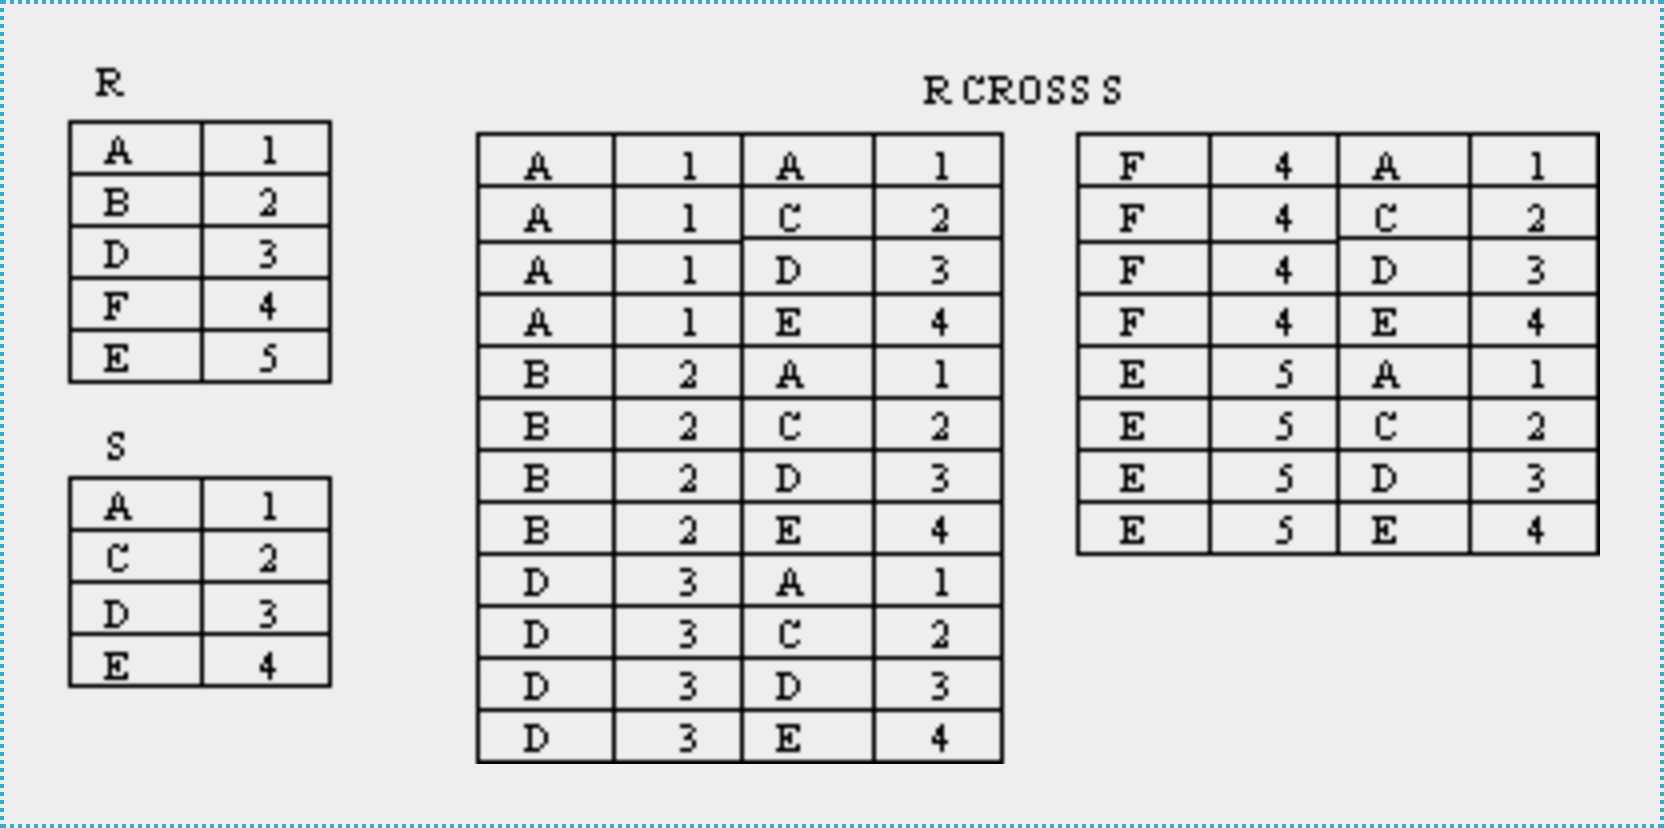
\includegraphics[width=0.8\linewidth]{figs/spm6/cartesianproduct}
\caption{Eksempel på \textit{cartesian product}.}
\label{fig:cartesian_product}
\end{figure}

Som det også kan ses i figur~\ref{fig:cartesian_product} så får hver attribut/kolonne i relation R sin \textit{egen udgave} af hver attribut/kolonne i relation S.